% ==============================================================================
% =================================== Aufgabe 2 =================================
% ==============================================================================

\chapter{Aufgabe}
\label{chap:2 Aufgabe}
\thispagestyle{fancy}
\section*{} 
\begin{figure}[h]
    \centering
    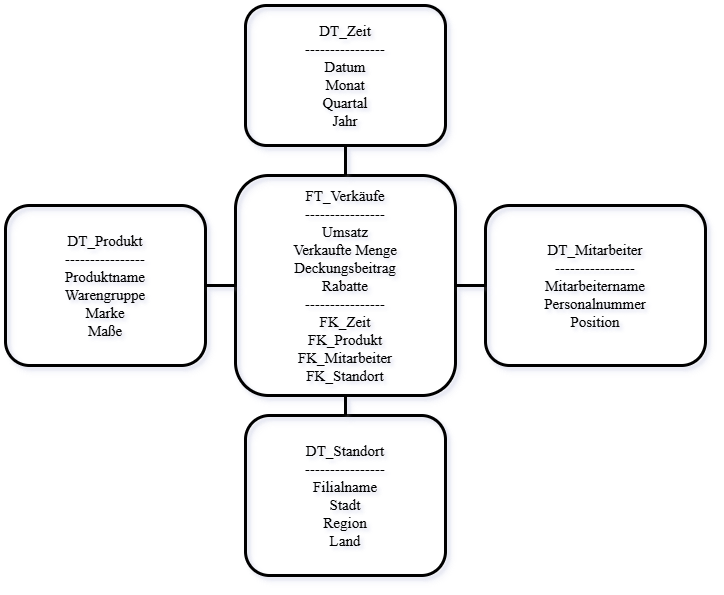
\includegraphics[width=0.95\textwidth]{./asset/image/Star-Schema.png}
    \caption{Star-Schema für Reseller-Umsatzanalyse}
    \label{fig:starschema}
    [Quelle: Eigene Darstellung]
\end{figure}
Wie in der von mir entworfenen \hyperref[fig:starschema]{Abbildung \ref{fig:starschema}} dargestellt, bildet die Faktentabelle das Herzstück des Schemas, umgeben von mehreren deskriptiven sternförmige \uline{Dimensionstabellen}. Wie Gattnar \cite[18]{15} in ihren Ausführungen zu Business-Intelligence-Datenbanken verdeutlicht, resultiert aus diesem Aufbau ein multidimensionales Datenmodell, das explizit auf die Anforderungen analytischer Abfragen hin optimiert wurde. \par Für das Szenario eines Resellers mit verschiedenen Standorten und lokalen Mitarbeitern lässt sich das Schema wie folgt entwerfen:
\begin{enumerate}[label=\arabic*.), leftmargin=*]
    \item \textbf{Die zentrale Faktentabelle (\textit{\acs{z. B.} \acs{FT}\_Verkäufe)}} \par Die Faktentabelle steht im Mittelpunkt und enthält die quantitativ messbaren Kennzahlen (\textit{Measures}) des Geschäftsbetriebs.
    \begin{itemize}
        \item \textbf{Measures (\textit{Kennzahlen}):}
        \begin{itemize}
            \item \textbf{Umsatz:} Der monetäre Wert der verkauften Produkte.
            \item \textbf{Verkaufte Menge:} Die Anzahl der abgesetzten Einheiten.
            \item \textbf{Deckungsbeitrag:} Errechnet aus Umsatz abzüglich variabler Kosten.
            \item \textbf{Rabatte:} Gewährte Preisnachlässe pro Verkaufsvorgang.
        \end{itemize}
        \item \textbf{Zusammengesetzter Primärschlüssel:} Besteht aus den Fremdschlüsseln der verknüpften Dimensionstabellen (\textit{Zeit}, \textit{Produkt}, \textit{Mitarbeiter}, \textit{Standort}).
    \end{itemize}
    \item \textbf{Die Dimensionstabellen (\textit{\acs{DT}})} \par Im Rahmen der methodischen Beschreibung des Star-Schemas betont Goram \cite[19]{16}, dass die Dimensionstabellen vor allem dazu dienen, beschreibende Attribute bereitzustellen, über welche die zentralen Fakten strukturiert gruppiert und analysiert werden können.
    \begin{itemize}
        \item \textbf{\acs{DT}\_Zeit (\textit{Zeitdimension}):} Ermöglicht Analysen über Zeiträume hinweg.
        \begin{itemize}
            \item Attribute: Datum, Monat, Quartal, Jahr.
        \end{itemize}
        \item \textbf{\acs{DT}\_Produkt (\textit{Produktdimension}):} Enthält Details zu den verkauften Waren. Die hier gewählte Aufteilung der Produktmerkmale in Kategorien wie \uline{Warengruppen} (\textit{Klassifizierungsmerkmale}) oder Marken stützt sich auf die von Gronau \cite[99]{17} dargelegte Notwendigkeit, vertriebsrelevante Stammdaten für eine effiziente Auswertung sinnvoll zu gruppieren.
        \begin{itemize}
            \item Attribute: Produktname, \uline{Warengruppe} (\textit{Klassifizierungsmerkmal}), Marke, Maße. Hierarchien innerhalb der Dimension (\textit{\acs{z. B.} Produkt -> Warengruppe -> Produkthierarchie}) sind möglich.
        \end{itemize}
        \item \textbf{\acs{DT}\_Mitarbeiter (\textit{Personaldimension}):} Bildet die lokale Belegschaft ab.
        \begin{itemize}
            \item Attribute: Mitarbeitername, Personalnummer, Funktion/Position.
        \end{itemize}
        \item \textbf{\acs{DT}\_Standort (\textit{Standortdimension}):} Spiegelt die verschiedenen Niederlassungen wider.
        \begin{itemize}
            \item Attribute: Filialname, Stadt, \uline{Region} (\textit{\acs{z. B.} Nord, Süd}), Land.
        \end{itemize}
    \end{itemize}
\end{enumerate}
\textbf{Beispielhafte Abfragestruktur} \par Mithilfe dieses Schemas kann der Reseller komplexe Analysefragen beantworten, wie \acs{z. B.}: \textit{„Welcher Umsatz wurde im letzten Quartal (Zeit) mit der Warengruppe 'Elektronik' (Produkt) am Standort 'Berlin' (Standort) von dem Mitarbeiter 'Max Mustermann' (Mitarbeiter) erzielt?“}. \par \textbf{Vorteile dieses Entwurfs:}
\begin{itemize}
    \item \textbf{Intuitive Bedienung:} Das Modell ist leicht verständlich für Endanwender in den Fachbereichen.
    \item \textbf{Performance:} Durch die geringe Anzahl an Join-Operationen (\textit{Verknüpfungen}) werden schnelle Abfrageergebnisse erzielt.
    \item \textbf{Hierarchieabbildung:} Innerhalb der Dimensionen (\textit{wie Standort oder Produkt}) können Navigationspfade zur Aggregation der Daten (\textit{Drill-down/Drill-up}) genutzt werden.
\end{itemize}

% ==============================================================================
% =================================== Aufgabe 2 =================================
% ==============================================================================